\chapter{Оценка на количество делителей числа и сверхсоставные числа}

\section{Предыстория и мотивация}

Иногда бывает так, что асимптотика решения задачи зависит от количества делителей числа во входе. Вы, возможно, слышали такое утверждение: <<количество делителей числа $n$~--- это примерно кубический корень из $n$>>. Действительно ли у чисел может быть так много делителей?

На самом деле, это, конечно, не так, но оценка в кубический корень дает нужный порядок величин для грубых оценок на числах, с которыми мы имеем дело в реальной жизни (отличие не больше, чем в $4$ раза при $n \le 10^{15}$, и не больше, чем в $10$ раз при $n \le 10^{18}$). Давайте разберемся, сколько все таки на самом деле делителей у чисел, и как этим пользоваться, а также придумаем новую более точную оценку.


\section{Субполиномиальность и сверхсоставные числа}

Будем обозначать количество делителей числа $n$ как $d(n)$. На самом деле $d(n)$~--- это субполиномиальная величина, то есть для достаточно больших $n$ она меньше $n^{\varepsilon}$ для сколь угодно малого положительного $\varepsilon$. С доказательством можно, к примеру, ознакомиться, в \href{https://codeforces.com/blog/entry/3863}{этой статье}. То есть для ооочень больших $n$ можно оценивать $d(n)$ не только как кубический корень, но и как корень четвертой, пятой... любой степени! Однако нас не очень сильно интересуют эти теоретические оценки, потому что по настоящему они достигаются только для невероятно огромных чисел, с которыми мы не работаем. Нас интересуют более практичные оценки.

Максимальное количество делителей неразрывно связано с таким понятием как <<сверхсоставные числа>> (highly composite numbers). Это такие числа, у которых больше делителей, чем у всех меньших чисел. Первые сверхсоставные числа~--- это $1, 2, 4, 6, 12, 24\ldots$ Тогда, к примеру, если мы хотим понять, какое максимальное количество делителей есть у чисел, не превосходящих $1000$, можно посмотреть в список сверхсоставных чисел, найти там самое больше число, не превосходящее $1000$ (это будет $840$), и посмотреть, сколько у него делителей ($32$). На удивление сверхсоставные числа встречаются не очень часто: существует всего $156$ сверхсоставных чисел, не превосходящих $10^{18}$. К примеру, сверхсоставные числа можно найти как последовательность на OEIS: \href{https://oeis.org/A002182}{oeis.org/A002182}.

\section{Быстрая генерация больших сверхсоставных чисел}

Для генерации сверхсоставных чисел есть \href{https://gist.github.com/dario2994/fb4713f252ca86c1254d}{этот замечательный скрипт}. По ссылке есть скрипт, способный очень быстро вычислить все сверхсоставные числа до \verb+MAXN+ (при \verb+MAXN+$=10^{100}$ программа работает меньше секунды), а также ниже представлен список всех всех сверхсоставных чисел до $10^{18}$ с их количествами делителей и разложениями.

Давайте разберемся, как же этому коду удается так быстро находить такие большие сверхсоставные числа. Для начала придумаем парочку очевидных алгоритмов поиска сверхсоставных чисел. Давайте идти по числам по возрастанию, находить их количества делителей, и если все меньшие числа имели меньше делителей, то новое число будет сверхсоставным. Количество делителей числа можно находить аналогично проверке на простоту за $O(\sqrt n)$ (все делители разбиваются на пары вида ($x$, $\frac{n}{x}$), и один из этих делителей будет не больше корня из $n$). В частности, из этого следует самая простая оценка на количество делителей числа: $d(n) \le 2 \cdot \sqrt n$. Тогда мы найдем все сверхсоставные числа до n за $O(n \cdot \sqrt n)$, что очень долго.

Более умный способ основан на полезной идее о том, что вместо того, чтобы для каждого числа перебирать делители, мы можем действовать наоборот: для каждого числа будем перебирать, какие числа на него делятся. Эта идея похожа на идею решета Эратосфена и, как известно, работает за $O(n \log n)$, потому что числа, делящиеся на $k$~--- это $k$,  $2k$, $3k$, $\ldots$ Их $\frac{n}{k}$ штук. Всего мы получим $\frac{n}{1} + \frac{n}{2} + \ldots + \frac{n}{n} = O(n \log n)$ (сумма гармонического ряда). В частности, из этого следует, что в среднем у чисел от $1$ до $n$ как раз таки очень мало делителей: $O(\log n)$. Но это все еще долго, такой алгоритм будет работать только для $n$ порядка $10^8$.

Для того, чтобы придумать эффективный алгоритм, давайте подробнее изучим нашу задачу. Давайте поймем, чему же равно количество делителей числа $n$. Пусть $n = p_1^{a_1} \cdot p_2^{a_2} \cdot \ldots \cdot p_k^{a_k}$. Тогда у $n$ есть ровно $(a_1 + 1) \cdot (a_2 + 1) \cdot \ldots \cdot (a_k + 1)$ делителей, потому что любой делитель $n$ должен состоять только из тех простых, которые есть в $n$, и при этом степени должны быть не больше, чем степени в $n$. Поэтому у нас есть $a_1 + 1$ вариантов степени $p_1$ (от $0$ до $a_1$), $a_2 + 1$ вариантов степени $p_2$ и так далее. Мы хотим, чтобы это произведение было как можно больше.

Несложно заметить, глядя на список по ссылке выше, что степени вхождения простых $2, 3, 5, 7 \ldots$ в сверхсоставные числа не возрастают. Действительно, если есть, к примеру, число $40 = 2^3 \cdot 3^0 \cdot 5^1$, то можно поменять местами степени тройки и пятерки и получить число $24 = 2^3 \cdot 3^1 \cdot 5^0$, у которого будет ровно столько же делителей, но само число будет меньше.

Собственно, ровно на этой идее и основан алгоритм выше. Он начинает с числа $1$ и постепенно генерирует все возможные числа, не превосходящие \verb+MAXN+, у которых степени вхождения простых не возрастают. Так как сумма степеней простых не больше логарифма \verb+MAXN+, таких невозрастающих наборов степеней будет не очень много. После чего, зная разложение, легко посчитать для каждого из них количество делителей. Однако это еще не ответ. Это лишь кандидаты на то, чтобы быть сверхсоставными. Остается отсортировать их и пройтись по порядку, выбирая все числа, у которых больше делителей, чем у всех предыдущих.

\section{Таблица для повседневного использования}

Список сверхсоставных чисел~--- это, конечно, хорошо, но он не очень удобен для использования на практике. На практике у нас есть некоторое ограничение на $n$, и мы хотим узнать, какое максимальное количество делителей может быть у числа с такими ограничениями. На этот случай есть такая замечательная табличка:

{
\newcommand\bn[1]{\multicolumn{1}{|c|}{#1}}
\newcommand\cn[1]{\multicolumn{1}{c|}{#1}}
\begin{center}
\begin{tabular}{|r|r|l|r|}
\hline
    \bn{$\le N$} & \cn{$n$} & \cn{Факторизация} & \cn{$d(n)$}
\\\hline
    20 & \num{12} & $2^2 \cdot 3^1$ & \num{6}
\\\hline
    50 & \num{48} & $2^4 \cdot 3^1$ & \num{10}
\\\hline
     100 & \num{60} & $2^2 \cdot 3^1 \cdot 5^1$ & \num{12}
\\\hline
    $10^3$ & \num{840} & $2^3 \cdot 3^1 \cdot 5^1 \cdot 7^1$ \strut & \num{32}
\\\hline
    $10^4$ & \num{7560} & $2^3 \cdot 3^3 \cdot 5^1 \cdot 7^1$ & \num{64}
\\\hline
    $10^5$ & \num{83160} & $2^3 \cdot 3^3 \cdot 5^1 \cdot 7^1 \cdot 11^1$ & \num{128}
\\\hline
    $10^6$ & \num{720720} & $2^4 \cdot 3^2 \cdot 5^1 \cdot 7^1 \cdot 11^1 \cdot 13^1$ & \num{240}
\\\hline
    $10^7$ & \num{8648640} & $2^6 \cdot 3^3 \cdot 5^1 \cdot 7^1 \cdot 11^1 \cdot 13^1$ & \num{448}
\\\hline
    $10^8$ & \num{73513440} & $2^5 \cdot 3^3 \cdot 5^1 \cdot 7^1 \cdot 11^1 \cdot 13^1 \cdot 17^1$ & \num{768}
\\\hline
    $10^9$ & \num{735134400} & $2^6 \cdot 3^3 \cdot 5^2 \cdot 7^1 \cdot 11^1 \cdot 13^1 \cdot 17^1$ & \num{1344}
\\\hline
    $10^{11}$ & \num{97772875200} & $2^6 \cdot 3^3 \cdot 5^2 \cdot 7^2 \cdot 11^1 \cdot 13^1 \cdot 17^1 \cdot 19^1$ & \num{4032}
\\\hline
    $10^{12}$ & \num{963761198400} & $2^6 \cdot 3^4 \cdot 5^2 \cdot 7^1 \cdot 11^1 \cdot 13^1 \cdot 17^1 \cdot 19^1 \cdot 23^1$ & \num{6720}
\\\hline
    $10^{15}$ & \num{866421317361600} & $2^6 \cdot 3^4 \cdot 5^2 \cdot 7^1 \cdot 11^1 \cdot 13^1 \cdot 17^1 \cdot 19^1 \cdot 23^1 \cdot 29^1 \cdot 31^1$ & \num{26880}
\\\hline
    $10^{18}$ & \num{897612484786617600} & $2^8 \cdot 3^4 \cdot 5^2 \cdot 7^2 \cdot 11^1 \cdot 13^1 \cdot 17^1 \cdot 19^1 \cdot 23^1 \cdot 29^1 \cdot 31^1 \cdot 37^1$ & \num{103680}
\\\hline
\end{tabular}
\end{center}
}

\graytext{Исходный код таблицы в \LaTeX \ доступен по \href{https://pastebin.com/T9HzdZSD}{ссылке}}

По первому столбцу можно понять ограничения, по второму столбцу можно увидеть наименьшее число с наибольшим количеством делителей, потом его разложение на простые, и последний столбец, наконец, говорит нам то самое количество делителей. Если у вас нет этой таблицы, ее можно, к примеру, получить по двум последовательностям OEIS: \href{http://oeis.org/A066150}{oeis.org/A066150}, \href{http://oeis.org/A066151}{oeis.org/A066151}.

\section{Численный анализ оценки в кубический корень}

Для точности рекомендуется пользоваться этой таблицей и не полагаться на оценку в кубический корень, однако если этой таблички нет под рукой, то эта оценка даст вам примерное представление о максимальном количестве делителей.

Чтобы лучше понимать эту оценку, давайте проанализируем графики:

\begin{center}    
% This file was created with tikzplotlib v0.9.15.
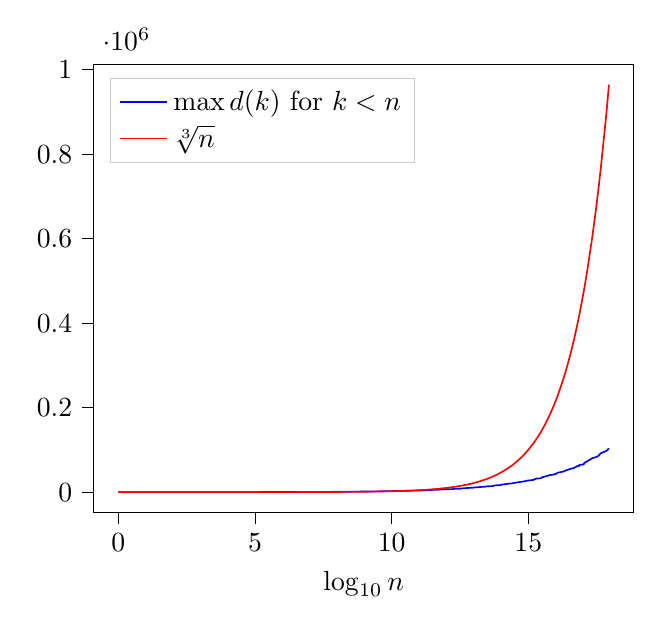
\begin{tikzpicture}

\begin{axis}[
legend cell align={left},
legend style={
  fill opacity=0.8,
  draw opacity=1,
  text opacity=1,
  at={(0.03,0.97)},
  anchor=north west,
  draw=white!80!black
},
tick align=outside,
tick pos=left,
x grid style={white!69.0196078431373!black},
xlabel={$\log_{10} n$},
xmin=-0.897654444225251, xmax=18.8507433287303,
xtick style={color=black},
y grid style={white!69.0196078431373!black},
ymin=-48230.6940091575, ymax=1012866.57419231,
ytick style={color=black}
]
\addplot [semithick, blue]
table {%
0 1
0.301029995663981 2
0.602059991327962 3
0.778151250383644 4
1.07918124604762 6
1.38021124171161 8
1.55630250076729 9
1.68124123737559 10
1.77815125038364 12
2.07918124604762 16
2.25527250510331 18
2.38021124171161 20
2.55630250076729 24
2.85733249643127 30
2.92427928606188 32
3.10037054511756 36
3.22530928172586 40
3.40140054078154 48
3.70243053644553 60
3.87852179550121 64
4.00346053210951 72
4.17955179116519 80
4.30449052777349 84
4.40140054078154 90
4.44279322593977 96
4.65667304588485 100
4.70243053644553 108
4.74382322160375 120
4.91991448065943 128
5.04485321726773 144
5.22094447632341 160
5.34588321293171 168
5.44279322593977 180
5.52197447198739 192
5.69806573104307 200
5.74382322160375 216
5.82300446765137 224
5.85776657391059 240
6.03385783296627 256
6.15879656957457 288
6.33488782863025 320
6.45982656523855 336
6.55673657824661 360
6.63591782429423 384
6.81200908334991 400
6.85776657391059 432
6.93694781995821 448
7.03385783296627 480
7.15879656957457 504
7.23797781562219 512
7.33488782863025 576
7.51097908768593 600
7.56533675000852 640
7.63591782429423 672
7.78718549962488 720
7.8663667456725 768
8.04245800472819 800
8.08821549528886 864
8.16739674133648 896
8.26430675434454 960
8.38924549095284 1008
8.46842673700047 1024
8.56533675000852 1152
8.7414280090642 1200
8.84409035096135 1280
8.8663667456725 1344
9.04245800472819 1440
9.14512034662533 1536
9.32121160568101 1600
9.34348800039217 1680
9.36696909624169 1728
9.44615034228931 1792
9.54306035529737 1920
9.66799909190567 2016
9.74718033795329 2048
9.84409035096135 2304
10.020181610017 2400
10.1451203466253 2688
10.321211605681 2880
10.4461503422893 3072
10.622241601345 3360
10.6891883909756 3456
10.8078781783069 3584
10.8652796500313 3600
10.904788191315 3840
10.9902183866396 4032
11.1089081739709 4096
11.1663096456953 4320
11.2058181869789 4608
11.3819094460346 4800
11.4673396413593 5040
11.5068481826429 5376
11.6829394416986 5760
11.8078781783069 6144
11.9839694373626 6720
12.0509162269932 6912
12.2058181869789 7168
12.2270074860489 7200
12.2849994330266 7680
12.3519462226572 8064
12.5068481826429 8192
12.5280374817129 8640
12.6529762183212 9216
12.8290674773768 10080
12.9540062139851 10368
12.9692461805419 10752
13.1300974730408 11520
13.2702761762059 12288
13.4311274687048 12960
13.4463674352615 13440
13.5133142248922 13824
13.6682161848779 14336
13.6894054839478 14400
13.7473974309255 15360
13.8143442205561 16128
13.9692461805419 16384
13.9904354796118 17280
14.1153742162201 18432
14.2914654752758 20160
14.4164042118841 20736
14.4606078743762 21504
14.5924954709398 23040
14.7616378700401 24576
14.8935254666038 25920
14.9377291290958 26880
15.0046759187264 27648
15.1595778787122 28672
15.1807671777821 28800
15.2387591247598 30720
15.3057059143904 32256
15.4606078743762 32768
15.4817971734461 34560
15.6067359100544 36864
15.7828271691101 40320
15.9077659057184 41472
16.0046759187264 43008
16.0838571647741 46080
16.2599484238297 48384
16.3057059143904 49152
16.384887160438 51840
16.4817971734461 53760
16.5609784194937 55296
16.685917156102 57600
16.7828271691101 61440
16.8620084151577 62208
16.8739076384574 64512
17.0288095984431 65536
17.0499988975131 69120
17.1749376341214 73728
17.3510288931771 80640
17.4759676297854 82944
17.5728776427934 86016
17.6520588888411 92160
17.8281501478967 96768
17.8739076384574 98304
17.953088884505 103680
};
\addlegendentry{$\max d(k)$ for $k < n$}
\addplot [semithick, red]
table {%
0 1
0.301029995663981 1.25992104989487
0.602059991327962 1.5874010519682
0.778151250383644 1.81712059283214
1.07918124604762 2.28942848510666
1.38021124171161 2.88449914061482
1.55630250076729 3.30192724889463
1.68124123737559 3.63424118566428
1.77815125038364 3.91486764116886
2.07918124604762 4.93242414866094
2.25527250510331 5.64621617328617
2.38021124171161 6.21446501190772
2.55630250076729 7.11378660898013
2.85733249643127 8.96280949311433
2.92427928606188 9.43538796063307
3.10037054511756 10.8008229825529
3.22530928172586 11.8878439055263
3.40140054078154 13.6081842319067
3.70243053644553 17.1452377646268
3.87852179550121 19.6263978611315
4.00346053210951 21.6016459651058
4.17955179116519 24.7277117988513
4.30449052777349 27.2163684638135
4.40140054078154 29.3179441775647
4.44279322593977 30.2643308005599
4.65667304588485 35.6635317165788
4.70243053644553 36.9382950089567
4.74382322160375 38.1306674366071
4.91991448065943 43.6487180927487
5.04485321726773 48.0416305499223
5.22094447632341 54.9939387259813
5.34588321293171 60.5286616011197
5.44279322593977 65.2025241473266
5.52197447198739 69.2880210174927
5.69806573104307 79.3149844970585
5.74382322160375 82.1500326794955
5.82300446765137 87.2974361854975
5.85776657391059 89.6579610096387
6.03385783296627 102.632744926025
6.15879656957457 112.961952366698
6.33488782863025 129.30915574079
6.45982656523855 142.323141624024
6.55673657824661 153.312956754559
6.63591782429423 162.919327261956
6.81200908334991 186.496074303968
6.85776657391059 193.162221436692
6.93694781995821 205.265489852049
7.03385783296627 221.115546001821
7.15879656957457 243.369148832542
7.23797781562219 258.618311481579
7.33488782863025 278.588130866693
7.51097908768593 318.903801209415
7.56533675000852 332.490251659851
7.63591782429423 350.999050329814
7.78718549962488 394.21078331238
7.8663667456725 418.911466951091
8.04245800472819 479.533922587823
8.08821549528886 496.674463990815
8.16739674133648 527.795375254019
8.26430675434454 568.550332842828
8.38924549095284 625.770612127281
8.46842673700047 664.980503319703
8.56533675000852 716.328532273415
8.7414280090642 819.991473240702
8.84409035096135 887.217535713122
8.8663667456725 902.517396451574
9.04245800472819 1033.12451787027
9.14512034662533 1117.82404908082
9.32121160568101 1279.58910965145
9.34348800039217 1301.65532722724
9.36696909624169 1325.32695859118
9.44615034228931 1408.37004951564
9.54306035529737 1517.12064553921
9.66799909190567 1669.80733312218
9.74718033795329 1774.43507142624
9.84409035096135 1911.45223654495
10.020181610017 2188.06659913343
10.1451203466253 2408.27890869162
10.321211605681 2756.79116682009
10.4461503422893 3034.24129107842
10.622241601345 3473.33922124088
10.6891883909756 3656.47658766686
10.8078781783069 4005.21707922945
10.8652796500313 4185.62082746506
10.904788191315 4314.48930830005
10.9902183866396 4606.87182124925
11.1089081739709 5046.25730751965
11.1663096456953 5273.55178740163
11.2058181869789 5435.91589907361
11.3819094460346 6222.57035099166
11.4673396413593 6644.25890465805
11.5068481826429 6848.82486670106
11.6829394416986 7839.94736966612
11.8078781783069 8628.97861660011
11.9839694373626 9877.71472111029
12.0509162269932 10398.5330302661
12.2058181869789 11711.32578506
12.2270074860489 11903.3488614069
12.2849994330266 12445.1407019833
12.3519462226572 13101.3306528594
12.5068481826429 14755.3458787737
12.5280374817129 14997.2797947287
12.6529762183212 16506.6422711705
12.8290674773768 18895.3885045417
12.9540062139851 20797.0660605322
12.9692461805419 21041.7598741413
13.1300974730408 23806.6977228138
13.2702761762059 26510.9561922639
13.4311274687048 29994.5595894574
13.4463674352615 30347.4691369919
13.5133142248922 31947.5879913366
13.6682161848779 35980.9032605285
13.6894054839478 36570.8589889088
13.7473974309255 38235.4151767311
13.8143442205561 40251.4386036537
13.9692461805419 45333.0974121709
13.9904354796118 46076.3950528634
14.1153742162201 50713.6347852944
14.2914654752758 58052.6200303745
14.4164042118841 63895.1759826732
14.4606078743762 66100.177360893
14.5924954709398 73141.7179778176
14.7616378700401 83281.0048587736
14.8935254666038 92152.7901057267
14.9377291290958 95332.9523959914
15.0046759187264 100359.534806556
15.1595778787122 113029.713358191
15.1807671777821 114882.988869092
15.2387591247598 120111.993472335
15.3057059143904 126445.090460438
15.4606078743762 142408.515123568
15.4817971734461 144743.495951007
15.6067359100544 159310.831126967
15.7828271691101 182365.377384048
15.9077659057184 200719.069613113
16.0046759187264 216218.063262708
16.0838571647741 229765.977738184
16.2599484238297 263016.387171091
16.3057059143904 272417.689272187
16.384887160438 289486.991902015
16.4817971734461 311840.40883334
16.5609784194937 331379.882664157
16.685917156102 364730.754768095
16.7828271691101 392894.295296948
16.8620084151577 417512.489680265
16.8739076384574 421343.09346562
17.0288095984431 474536.765955206
17.0499988975131 482317.440091575
17.1749376341214 530859.032685157
17.3510288931771 607681.895502784
17.4759676297854 668840.46980686
17.5728776427934 720486.555124561
17.6520588888411 765631.211783974
17.8281501478967 876428.952672482
17.8739076384574 907756.176967677
17.953088884505 964634.880183149
};
\addlegendentry{$\sqrt[3]{n}$}
\end{axis}

\end{tikzpicture}


\end{center}

На данном графике на оси $X$ отложены десятичные логарифмы $n$ (то есть количество цифр в числе $n$), красный график~--- это кубический корень, а синий график~--- это максимальное количество делителей среди чисел, меньших $n$ (обратите внимание, что все числа по оси $Y$ умножаются на миллион). Из-за экспоненциального роста не видно, что происходит для чисел, меньших $10^{11}$, но и так видно, что для больших $n$ кубический корень уходит сильно выше, но все равно отношение не больше $10$ для обозримых чисел.

Давайте ограничим наш график на числа, меньшие $10^{12}$, чтобы посмотреть внимательнее на эту часть графика:

\begin{center}    
% This file was created with tikzplotlib v0.9.15.
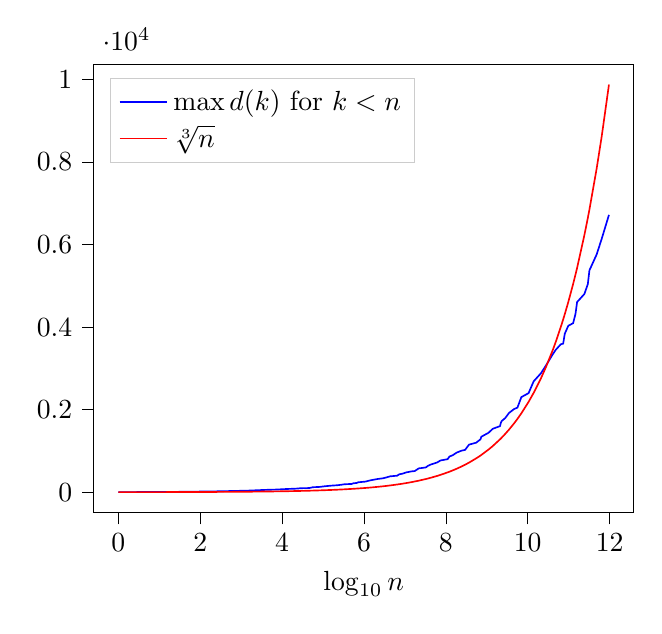
\begin{tikzpicture}

\begin{axis}[
legend cell align={left},
legend style={
  fill opacity=0.8,
  draw opacity=1,
  text opacity=1,
  at={(0.03,0.97)},
  anchor=north west,
  draw=white!80!black
},
tick align=outside,
tick pos=left,
x grid style={white!69.0196078431373!black},
xlabel={$\log_{10} n$},
xmin=-0.599198471868129, xmax=12.5831679092307,
xtick style={color=black},
y grid style={white!69.0196078431373!black},
ymin=-492.835736055515, ymax=10371.5504571658,
ytick style={color=black}
]
\addplot [semithick, blue]
table {%
0 1
0.301029995663981 2
0.602059991327962 3
0.778151250383644 4
1.07918124604762 6
1.38021124171161 8
1.55630250076729 9
1.68124123737559 10
1.77815125038364 12
2.07918124604762 16
2.25527250510331 18
2.38021124171161 20
2.55630250076729 24
2.85733249643127 30
2.92427928606188 32
3.10037054511756 36
3.22530928172586 40
3.40140054078154 48
3.70243053644553 60
3.87852179550121 64
4.00346053210951 72
4.17955179116519 80
4.30449052777349 84
4.40140054078154 90
4.44279322593977 96
4.65667304588485 100
4.70243053644553 108
4.74382322160375 120
4.91991448065943 128
5.04485321726773 144
5.22094447632341 160
5.34588321293171 168
5.44279322593977 180
5.52197447198739 192
5.69806573104307 200
5.74382322160375 216
5.82300446765137 224
5.85776657391059 240
6.03385783296627 256
6.15879656957457 288
6.33488782863025 320
6.45982656523855 336
6.55673657824661 360
6.63591782429423 384
6.81200908334991 400
6.85776657391059 432
6.93694781995821 448
7.03385783296627 480
7.15879656957457 504
7.23797781562219 512
7.33488782863025 576
7.51097908768593 600
7.56533675000852 640
7.63591782429423 672
7.78718549962488 720
7.8663667456725 768
8.04245800472819 800
8.08821549528886 864
8.16739674133648 896
8.26430675434454 960
8.38924549095284 1008
8.46842673700047 1024
8.56533675000852 1152
8.7414280090642 1200
8.84409035096135 1280
8.8663667456725 1344
9.04245800472819 1440
9.14512034662533 1536
9.32121160568101 1600
9.34348800039217 1680
9.36696909624169 1728
9.44615034228931 1792
9.54306035529737 1920
9.66799909190567 2016
9.74718033795329 2048
9.84409035096135 2304
10.020181610017 2400
10.1451203466253 2688
10.321211605681 2880
10.4461503422893 3072
10.622241601345 3360
10.6891883909756 3456
10.8078781783069 3584
10.8652796500313 3600
10.904788191315 3840
10.9902183866396 4032
11.1089081739709 4096
11.1663096456953 4320
11.2058181869789 4608
11.3819094460346 4800
11.4673396413593 5040
11.5068481826429 5376
11.6829394416986 5760
11.8078781783069 6144
11.9839694373626 6720
};
\addlegendentry{$\max d(k)$ for $k < n$}
\addplot [semithick, red]
table {%
0 1
0.301029995663981 1.25992104989487
0.602059991327962 1.5874010519682
0.778151250383644 1.81712059283214
1.07918124604762 2.28942848510666
1.38021124171161 2.88449914061482
1.55630250076729 3.30192724889463
1.68124123737559 3.63424118566428
1.77815125038364 3.91486764116886
2.07918124604762 4.93242414866094
2.25527250510331 5.64621617328617
2.38021124171161 6.21446501190772
2.55630250076729 7.11378660898013
2.85733249643127 8.96280949311433
2.92427928606188 9.43538796063307
3.10037054511756 10.8008229825529
3.22530928172586 11.8878439055263
3.40140054078154 13.6081842319067
3.70243053644553 17.1452377646268
3.87852179550121 19.6263978611315
4.00346053210951 21.6016459651058
4.17955179116519 24.7277117988513
4.30449052777349 27.2163684638135
4.40140054078154 29.3179441775647
4.44279322593977 30.2643308005599
4.65667304588485 35.6635317165788
4.70243053644553 36.9382950089567
4.74382322160375 38.1306674366071
4.91991448065943 43.6487180927487
5.04485321726773 48.0416305499223
5.22094447632341 54.9939387259813
5.34588321293171 60.5286616011197
5.44279322593977 65.2025241473266
5.52197447198739 69.2880210174927
5.69806573104307 79.3149844970585
5.74382322160375 82.1500326794955
5.82300446765137 87.2974361854975
5.85776657391059 89.6579610096387
6.03385783296627 102.632744926025
6.15879656957457 112.961952366698
6.33488782863025 129.30915574079
6.45982656523855 142.323141624024
6.55673657824661 153.312956754559
6.63591782429423 162.919327261956
6.81200908334991 186.496074303968
6.85776657391059 193.162221436692
6.93694781995821 205.265489852049
7.03385783296627 221.115546001821
7.15879656957457 243.369148832542
7.23797781562219 258.618311481579
7.33488782863025 278.588130866693
7.51097908768593 318.903801209415
7.56533675000852 332.490251659851
7.63591782429423 350.999050329814
7.78718549962488 394.21078331238
7.8663667456725 418.911466951091
8.04245800472819 479.533922587823
8.08821549528886 496.674463990815
8.16739674133648 527.795375254019
8.26430675434454 568.550332842828
8.38924549095284 625.770612127281
8.46842673700047 664.980503319703
8.56533675000852 716.328532273415
8.7414280090642 819.991473240702
8.84409035096135 887.217535713122
8.8663667456725 902.517396451574
9.04245800472819 1033.12451787027
9.14512034662533 1117.82404908082
9.32121160568101 1279.58910965145
9.34348800039217 1301.65532722724
9.36696909624169 1325.32695859118
9.44615034228931 1408.37004951564
9.54306035529737 1517.12064553921
9.66799909190567 1669.80733312218
9.74718033795329 1774.43507142624
9.84409035096135 1911.45223654495
10.020181610017 2188.06659913343
10.1451203466253 2408.27890869162
10.321211605681 2756.79116682009
10.4461503422893 3034.24129107842
10.622241601345 3473.33922124088
10.6891883909756 3656.47658766686
10.8078781783069 4005.21707922945
10.8652796500313 4185.62082746506
10.904788191315 4314.48930830005
10.9902183866396 4606.87182124925
11.1089081739709 5046.25730751965
11.1663096456953 5273.55178740163
11.2058181869789 5435.91589907361
11.3819094460346 6222.57035099166
11.4673396413593 6644.25890465805
11.5068481826429 6848.82486670106
11.6829394416986 7839.94736966612
11.8078781783069 8628.97861660011
11.9839694373626 9877.71472111029
};
\addlegendentry{$\sqrt[3]{n}$}
\end{axis}

\end{tikzpicture}


\end{center}

Видно, что для маленьких чисел количество делителей все таки больше кубического корня, а где-то в районе между $10^{10}$ и $10^{11}$ эти графики меняются местами и уже никогда не встречаются вновь. Как я говорил раньше, сильный всплеск отношения между этими графиками происходит уже на очень больших числах, и для $n \le 10^{15}$ отношение между этими величинами не превосходит $4$.

Но если мы смотрим на такие графики, то мы видим только то, что происходит для больших чисел, потому что все маленькие величины становятся просто точкой. Для того, чтобы так не происходило, прологарифмируем также и ось $Y$:

\begin{center}    
% This file was created with tikzplotlib v0.9.15.
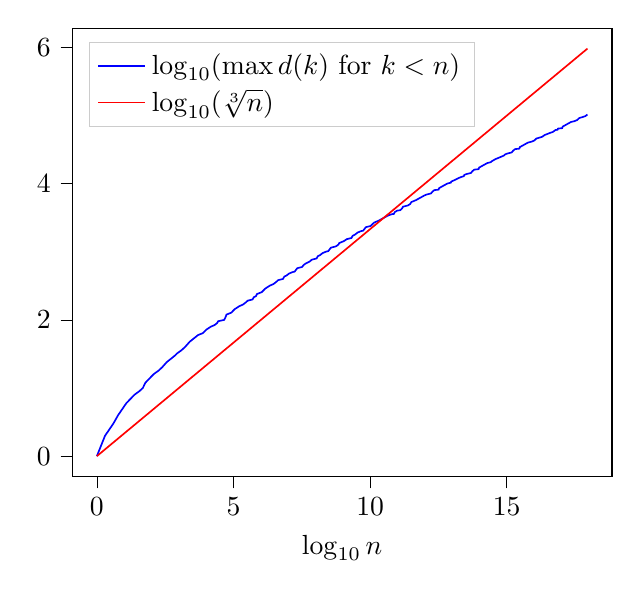
\begin{tikzpicture}

\begin{axis}[
legend cell align={left},
legend style={
  fill opacity=0.8,
  draw opacity=1,
  text opacity=1,
  at={(0.03,0.97)},
  anchor=north west,
  draw=white!80!black
},
tick align=outside,
tick pos=left,
x grid style={white!69.0196078431373!black},
xlabel={$\log_{10} n$},
xmin=-0.897654444225251, xmax=18.8507433287303,
xtick style={color=black},
y grid style={white!69.0196078431373!black},
ymin=-0.299218148075084, ymax=6.28358110957676,
ytick style={color=black}
]
\addplot [semithick, blue]
table {%
0 0
0.301029995663981 0.301029995663981
0.602059991327962 0.477121254719662
0.778151250383644 0.602059991327962
1.07918124604762 0.778151250383644
1.38021124171161 0.903089986991943
1.55630250076729 0.954242509439325
1.68124123737559 1
1.77815125038364 1.07918124604762
2.07918124604762 1.20411998265592
2.25527250510331 1.25527250510331
2.38021124171161 1.30102999566398
2.55630250076729 1.38021124171161
2.85733249643127 1.47712125471966
2.92427928606188 1.50514997831991
3.10037054511756 1.55630250076729
3.22530928172586 1.60205999132796
3.40140054078154 1.68124123737559
3.70243053644553 1.77815125038364
3.87852179550121 1.80617997398389
4.00346053210951 1.85733249643127
4.17955179116519 1.90308998699194
4.30449052777349 1.92427928606188
4.40140054078154 1.95424250943932
4.44279322593977 1.98227123303957
4.65667304588485 2
4.70243053644553 2.03342375548695
4.74382322160375 2.07918124604762
4.91991448065943 2.10720996964787
5.04485321726773 2.15836249209525
5.22094447632341 2.20411998265592
5.34588321293171 2.22530928172586
5.44279322593977 2.25527250510331
5.52197447198739 2.28330122870355
5.69806573104307 2.30102999566398
5.74382322160375 2.33445375115093
5.82300446765137 2.35024801833416
5.85776657391059 2.38021124171161
6.03385783296627 2.40823996531185
6.15879656957457 2.45939248775923
6.33488782863025 2.50514997831991
6.45982656523855 2.52633927738984
6.55673657824661 2.55630250076729
6.63591782429423 2.58433122436753
6.81200908334991 2.60205999132796
6.85776657391059 2.63548374681491
6.93694781995821 2.65127801399814
7.03385783296627 2.68124123737559
7.15879656957457 2.70243053644553
7.23797781562219 2.70926996097583
7.33488782863025 2.76042248342321
7.51097908768593 2.77815125038364
7.56533675000852 2.80617997398389
7.63591782429423 2.82736927305382
7.78718549962488 2.85733249643127
7.8663667456725 2.88536122003151
8.04245800472819 2.90308998699194
8.08821549528886 2.93651374247889
8.16739674133648 2.95230800966212
8.26430675434454 2.98227123303957
8.38924549095284 3.00346053210951
8.46842673700047 3.01029995663981
8.56533675000852 3.06145247908719
8.7414280090642 3.07918124604762
8.84409035096135 3.10720996964787
8.8663667456725 3.12839926871781
9.04245800472819 3.15836249209525
9.14512034662533 3.18639121569549
9.32121160568101 3.20411998265592
9.34348800039217 3.22530928172586
9.36696909624169 3.23754373814287
9.44615034228931 3.25333800532611
9.54306035529737 3.28330122870355
9.66799909190567 3.30449052777349
9.74718033795329 3.31132995230379
9.84409035096135 3.36248247475117
10.020181610017 3.38021124171161
10.1451203466253 3.42942926438179
10.321211605681 3.45939248775923
10.4461503422893 3.48742121135947
10.622241601345 3.52633927738984
10.6891883909756 3.53857373380686
10.8078781783069 3.55436800099009
10.8652796500313 3.55630250076729
10.904788191315 3.58433122436753
10.9902183866396 3.60552052343747
11.1089081739709 3.61235994796777
11.1663096456953 3.63548374681491
11.2058181869789 3.66351247041516
11.3819094460346 3.68124123737559
11.4673396413593 3.70243053644553
11.5068481826429 3.73045926004577
11.6829394416986 3.76042248342321
11.8078781783069 3.78845120702346
11.9839694373626 3.82736927305382
12.0509162269932 3.83960372947084
12.2058181869789 3.85539799665407
12.2270074860489 3.85733249643127
12.2849994330266 3.88536122003151
12.3519462226572 3.90655051910145
12.5068481826429 3.91338994363175
12.5280374817129 3.93651374247889
12.6529762183212 3.96454246607914
12.8290674773768 4.00346053210951
12.9540062139851 4.01569498852652
12.9692461805419 4.03148925570975
13.1300974730408 4.06145247908719
13.2702761762059 4.08948120268744
13.4311274687048 4.11260500153457
13.4463674352615 4.12839926871781
13.5133142248922 4.14063372513482
13.6682161848779 4.15642799231805
13.6894054839478 4.15836249209525
13.7473974309255 4.18639121569549
13.8143442205561 4.20758051476543
13.9692461805419 4.21441993929574
13.9904354796118 4.23754373814287
14.1153742162201 4.26557246174312
14.2914654752758 4.30449052777349
14.4164042118841 4.3167249841905
14.4606078743762 4.33251925137373
14.5924954709398 4.36248247475117
14.7616378700401 4.39051119835142
14.8935254666038 4.41363499719855
14.9377291290958 4.42942926438179
15.0046759187264 4.4416637207988
15.1595778787122 4.45745798798203
15.1807671777821 4.45939248775923
15.2387591247598 4.48742121135947
15.3057059143904 4.50861051042941
15.4606078743762 4.51544993495972
15.4817971734461 4.53857373380685
15.6067359100544 4.5666024574071
15.7828271691101 4.60552052343747
15.9077659057184 4.61775497985448
16.0046759187264 4.63354924703771
16.0838571647741 4.66351247041516
16.2599484238297 4.68470176948509
16.3057059143904 4.6915411940154
16.384887160438 4.71466499286254
16.4817971734461 4.73045926004577
16.5609784194937 4.74269371646278
16.685917156102 4.76042248342321
16.7828271691101 4.78845120702345
16.8620084151577 4.79384623891016
16.8739076384574 4.80964050609339
17.0288095984431 4.8164799306237
17.0499988975131 4.83960372947084
17.1749376341214 4.86763245307108
17.3510288931771 4.90655051910145
17.4759676297854 4.91878497551846
17.5728776427934 4.93457924270169
17.6520588888411 4.96454246607914
17.8281501478967 4.98573176514907
17.8739076384574 4.99257118967938
17.953088884505 5.01569498852652
};
\addlegendentry{$\log_{10}(\max d(k)$ for $k < n$)}
\addplot [semithick, red]
table {%
0 0
0.301029995663981 0.100343331887994
0.602059991327962 0.200686663775987
0.778151250383644 0.259383750127881
1.07918124604762 0.359727082015875
1.38021124171161 0.460070413903869
1.55630250076729 0.518767500255762
1.68124123737559 0.560413745791862
1.77815125038364 0.592717083461214
2.07918124604762 0.693060415349208
2.25527250510331 0.751757501701102
2.38021124171161 0.793403747237202
2.55630250076729 0.852100833589096
2.85733249643127 0.952444165477089
2.92427928606188 0.974759762020627
3.10037054511756 1.03345684837252
3.22530928172586 1.07510309390862
3.40140054078154 1.13380018026051
3.70243053644553 1.23414351214851
3.87852179550121 1.2928405985004
4.00346053210951 1.3344868440365
4.17955179116519 1.3931839303884
4.30449052777349 1.4348301759245
4.40140054078154 1.46713351359385
4.44279322593977 1.48093107531326
4.65667304588485 1.55222434862828
4.70243053644553 1.56747684548184
4.74382322160375 1.58127440720125
4.91991448065943 1.63997149355314
5.04485321726773 1.68161773908924
5.22094447632341 1.74031482544114
5.34588321293171 1.78196107097724
5.44279322593977 1.81426440864659
5.52197447198739 1.84065815732913
5.69806573104307 1.89935524368102
5.74382322160375 1.91460774053458
5.82300446765137 1.94100148921712
5.85776657391059 1.9525888579702
6.03385783296627 2.01128594432209
6.15879656957457 2.05293218985819
6.33488782863025 2.11162927621008
6.45982656523855 2.15327552174618
6.55673657824661 2.18557885941554
6.63591782429423 2.21197260809808
6.81200908334991 2.27066969444997
6.85776657391059 2.28592219130353
6.93694781995821 2.31231593998607
7.03385783296627 2.34461927765542
7.15879656957457 2.38626552319152
7.23797781562219 2.41265927187406
7.33488782863025 2.44496260954342
7.51097908768593 2.50365969589531
7.56533675000852 2.52177891666951
7.63591782429423 2.54530594143141
7.78718549962488 2.59572849987496
7.8663667456725 2.6221222485575
8.04245800472819 2.68081933490939
8.08821549528886 2.69607183176295
8.16739674133648 2.72246558044549
8.26430675434454 2.75476891811485
8.38924549095284 2.79641516365095
8.46842673700047 2.82280891233349
8.56533675000852 2.85511225000284
8.7414280090642 2.91380933635473
8.84409035096135 2.94803011698712
8.8663667456725 2.95545558189083
9.04245800472819 3.01415266824273
9.14512034662533 3.04837344887511
9.32121160568101 3.107070535227
9.34348800039217 3.11449600013072
9.36696909624169 3.12232303208056
9.44615034228931 3.1487167807631
9.54306035529737 3.18102011843246
9.66799909190567 3.22266636396856
9.74718033795329 3.2490601126511
9.84409035096135 3.28136345032045
10.020181610017 3.34006053667234
10.1451203466253 3.38170678220844
10.321211605681 3.44040386856034
10.4461503422893 3.48205011409644
10.622241601345 3.54074720044833
10.6891883909756 3.56306279699187
10.8078781783069 3.60262605943564
10.8652796500313 3.62175988334376
10.904788191315 3.63492939710499
10.9902183866396 3.66340612887986
11.1089081739709 3.70296939132363
11.1663096456953 3.72210321523176
11.2058181869789 3.73527272899298
11.3819094460346 3.79396981534487
11.4673396413593 3.82244654711975
11.5068481826429 3.83561606088098
11.6829394416986 3.89431314723287
11.8078781783069 3.93595939276897
11.9839694373626 3.99465647912086
12.0509162269932 4.0169720756644
12.2058181869789 4.06860606232631
12.2270074860489 4.07566916201629
12.2849994330266 4.09499981100886
12.3519462226572 4.11731540755239
12.5068481826429 4.16894939421431
12.5280374817129 4.17601249390429
12.6529762183212 4.21765873944039
12.8290674773768 4.27635582579228
12.9540062139851 4.31800207132838
12.9692461805419 4.32308206018063
13.1300974730408 4.37669915768027
13.2702761762059 4.42342539206862
13.4311274687048 4.47704248956827
13.4463674352615 4.48212247842051
13.5133142248922 4.50443807496405
13.6682161848779 4.55607206162597
13.6894054839478 4.56313516131595
13.7473974309255 4.58246581030851
13.8143442205561 4.60478140685205
13.9692461805419 4.65641539351396
13.9904354796118 4.66347849320394
14.1153742162201 4.70512473874004
14.2914654752758 4.76382182509193
14.4164042118841 4.80546807062803
14.4606078743762 4.82020262479205
14.5924954709398 4.86416515697993
14.7616378700401 4.92054595668005
14.8935254666038 4.96450848886792
14.9377291290958 4.97924304303194
15.0046759187264 5.00155863957548
15.1595778787122 5.05319262623739
15.1807671777821 5.06025572592737
15.2387591247598 5.07958637491993
15.3057059143904 5.10190197146347
15.4606078743762 5.15353595812539
15.4817971734461 5.16059905781536
15.6067359100544 5.20224530335146
15.7828271691101 5.26094238970336
15.9077659057184 5.30258863523946
16.0046759187264 5.33489197290881
16.0838571647741 5.36128572159135
16.2599484238297 5.41998280794324
16.3057059143904 5.4352353047968
16.384887160438 5.46162905347934
16.4817971734461 5.4939323911487
16.5609784194937 5.52032613983124
16.685917156102 5.56197238536734
16.7828271691101 5.59427572303669
16.8620084151577 5.62066947171923
16.8739076384574 5.6246358794858
17.0288095984431 5.67626986614772
17.0499988975131 5.6833329658377
17.1749376341214 5.7249792113738
17.3510288931771 5.78367629772569
17.4759676297854 5.82532254326179
17.5728776427934 5.85762588093114
17.6520588888411 5.88401962961368
17.8281501478967 5.94271671596558
17.8739076384574 5.95796921281914
17.953088884505 5.98436296150168
};
\addlegendentry{$\log_{10}(\sqrt[3]{n})$}
\end{axis}

\end{tikzpicture}


\end{center}

Теперь происходящее стало еще понятнее.

\section{Более точная практическая оценка}

Как мы уже говорили раньше, оценка в кубический корень очень проста и дает правильный порядок величин, когда нет доступа к таблице. Кроме того, кубический корень достаточно легко вычислить даже без компьютера. Однако если у вас нет таблицы, но при этом есть компьютер, я рекомендую вам другую очень точную оценку на максимальное количество делителей: $\exp((\ln \ln n)^{1.8})$.

\begin{center}    
% This file was created with tikzplotlib v0.9.15.
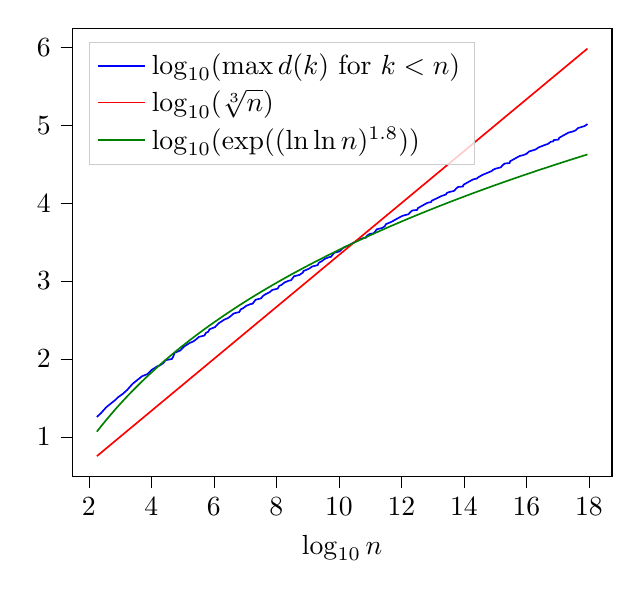
\begin{tikzpicture}

\begin{axis}[
legend cell align={left},
legend style={
  fill opacity=0.8,
  draw opacity=1,
  text opacity=1,
  at={(0.03,0.97)},
  anchor=north west,
  draw=white!80!black
},
tick align=outside,
tick pos=left,
x grid style={white!69.0196078431373!black},
xlabel={$\log_{10} n$},
xmin=1.47038168613322, xmax=18.7379797034751,
xtick style={color=black},
y grid style={white!69.0196078431373!black},
ymin=0.490127228711073, ymax=6.24599323449171,
ytick style={color=black}
]
\addplot [semithick, blue]
table {%
2.25527250510331 1.25527250510331
2.38021124171161 1.30102999566398
2.55630250076729 1.38021124171161
2.85733249643127 1.47712125471966
2.92427928606188 1.50514997831991
3.10037054511756 1.55630250076729
3.22530928172586 1.60205999132796
3.40140054078154 1.68124123737559
3.70243053644553 1.77815125038364
3.87852179550121 1.80617997398389
4.00346053210951 1.85733249643127
4.17955179116519 1.90308998699194
4.30449052777349 1.92427928606188
4.40140054078154 1.95424250943932
4.44279322593977 1.98227123303957
4.65667304588485 2
4.70243053644553 2.03342375548695
4.74382322160375 2.07918124604762
4.91991448065943 2.10720996964787
5.04485321726773 2.15836249209525
5.22094447632341 2.20411998265592
5.34588321293171 2.22530928172586
5.44279322593977 2.25527250510331
5.52197447198739 2.28330122870355
5.69806573104307 2.30102999566398
5.74382322160375 2.33445375115093
5.82300446765137 2.35024801833416
5.85776657391059 2.38021124171161
6.03385783296627 2.40823996531185
6.15879656957457 2.45939248775923
6.33488782863025 2.50514997831991
6.45982656523855 2.52633927738984
6.55673657824661 2.55630250076729
6.63591782429423 2.58433122436753
6.81200908334991 2.60205999132796
6.85776657391059 2.63548374681491
6.93694781995821 2.65127801399814
7.03385783296627 2.68124123737559
7.15879656957457 2.70243053644553
7.23797781562219 2.70926996097583
7.33488782863025 2.76042248342321
7.51097908768593 2.77815125038364
7.56533675000852 2.80617997398389
7.63591782429423 2.82736927305382
7.78718549962488 2.85733249643127
7.8663667456725 2.88536122003151
8.04245800472819 2.90308998699194
8.08821549528886 2.93651374247889
8.16739674133648 2.95230800966212
8.26430675434454 2.98227123303957
8.38924549095284 3.00346053210951
8.46842673700047 3.01029995663981
8.56533675000852 3.06145247908719
8.7414280090642 3.07918124604762
8.84409035096135 3.10720996964787
8.8663667456725 3.12839926871781
9.04245800472819 3.15836249209525
9.14512034662533 3.18639121569549
9.32121160568101 3.20411998265592
9.34348800039217 3.22530928172586
9.36696909624169 3.23754373814287
9.44615034228931 3.25333800532611
9.54306035529737 3.28330122870355
9.66799909190567 3.30449052777349
9.74718033795329 3.31132995230379
9.84409035096135 3.36248247475117
10.020181610017 3.38021124171161
10.1451203466253 3.42942926438179
10.321211605681 3.45939248775923
10.4461503422893 3.48742121135947
10.622241601345 3.52633927738984
10.6891883909756 3.53857373380686
10.8078781783069 3.55436800099009
10.8652796500313 3.55630250076729
10.904788191315 3.58433122436753
10.9902183866396 3.60552052343747
11.1089081739709 3.61235994796777
11.1663096456953 3.63548374681491
11.2058181869789 3.66351247041516
11.3819094460346 3.68124123737559
11.4673396413593 3.70243053644553
11.5068481826429 3.73045926004577
11.6829394416986 3.76042248342321
11.8078781783069 3.78845120702346
11.9839694373626 3.82736927305382
12.0509162269932 3.83960372947084
12.2058181869789 3.85539799665407
12.2270074860489 3.85733249643127
12.2849994330266 3.88536122003151
12.3519462226572 3.90655051910145
12.5068481826429 3.91338994363175
12.5280374817129 3.93651374247889
12.6529762183212 3.96454246607914
12.8290674773768 4.00346053210951
12.9540062139851 4.01569498852652
12.9692461805419 4.03148925570975
13.1300974730408 4.06145247908719
13.2702761762059 4.08948120268744
13.4311274687048 4.11260500153457
13.4463674352615 4.12839926871781
13.5133142248922 4.14063372513482
13.6682161848779 4.15642799231805
13.6894054839478 4.15836249209525
13.7473974309255 4.18639121569549
13.8143442205561 4.20758051476543
13.9692461805419 4.21441993929574
13.9904354796118 4.23754373814287
14.1153742162201 4.26557246174312
14.2914654752758 4.30449052777349
14.4164042118841 4.3167249841905
14.4606078743762 4.33251925137373
14.5924954709398 4.36248247475117
14.7616378700401 4.39051119835142
14.8935254666038 4.41363499719855
14.9377291290958 4.42942926438179
15.0046759187264 4.4416637207988
15.1595778787122 4.45745798798203
15.1807671777821 4.45939248775923
15.2387591247598 4.48742121135947
15.3057059143904 4.50861051042941
15.4606078743762 4.51544993495972
15.4817971734461 4.53857373380685
15.6067359100544 4.5666024574071
15.7828271691101 4.60552052343747
15.9077659057184 4.61775497985448
16.0046759187264 4.63354924703771
16.0838571647741 4.66351247041516
16.2599484238297 4.68470176948509
16.3057059143904 4.6915411940154
16.384887160438 4.71466499286254
16.4817971734461 4.73045926004577
16.5609784194937 4.74269371646278
16.685917156102 4.76042248342321
16.7828271691101 4.78845120702345
16.8620084151577 4.79384623891016
16.8739076384574 4.80964050609339
17.0288095984431 4.8164799306237
17.0499988975131 4.83960372947084
17.1749376341214 4.86763245307108
17.3510288931771 4.90655051910145
17.4759676297854 4.91878497551846
17.5728776427934 4.93457924270169
17.6520588888411 4.96454246607914
17.8281501478967 4.98573176514907
17.8739076384574 4.99257118967938
17.953088884505 5.01569498852652
};
\addlegendentry{$\log_{10}(\max d(k)$ for $k < n)$}
\addplot [semithick, red]
table {%
2.25527250510331 0.751757501701102
2.38021124171161 0.793403747237202
2.55630250076729 0.852100833589096
2.85733249643127 0.952444165477089
2.92427928606188 0.974759762020627
3.10037054511756 1.03345684837252
3.22530928172586 1.07510309390862
3.40140054078154 1.13380018026051
3.70243053644553 1.23414351214851
3.87852179550121 1.2928405985004
4.00346053210951 1.3344868440365
4.17955179116519 1.3931839303884
4.30449052777349 1.4348301759245
4.40140054078154 1.46713351359385
4.44279322593977 1.48093107531326
4.65667304588485 1.55222434862828
4.70243053644553 1.56747684548184
4.74382322160375 1.58127440720125
4.91991448065943 1.63997149355314
5.04485321726773 1.68161773908924
5.22094447632341 1.74031482544114
5.34588321293171 1.78196107097724
5.44279322593977 1.81426440864659
5.52197447198739 1.84065815732913
5.69806573104307 1.89935524368102
5.74382322160375 1.91460774053458
5.82300446765137 1.94100148921712
5.85776657391059 1.9525888579702
6.03385783296627 2.01128594432209
6.15879656957457 2.05293218985819
6.33488782863025 2.11162927621008
6.45982656523855 2.15327552174618
6.55673657824661 2.18557885941554
6.63591782429423 2.21197260809808
6.81200908334991 2.27066969444997
6.85776657391059 2.28592219130353
6.93694781995821 2.31231593998607
7.03385783296627 2.34461927765542
7.15879656957457 2.38626552319152
7.23797781562219 2.41265927187406
7.33488782863025 2.44496260954342
7.51097908768593 2.50365969589531
7.56533675000852 2.52177891666951
7.63591782429423 2.54530594143141
7.78718549962488 2.59572849987496
7.8663667456725 2.6221222485575
8.04245800472819 2.68081933490939
8.08821549528886 2.69607183176295
8.16739674133648 2.72246558044549
8.26430675434454 2.75476891811485
8.38924549095284 2.79641516365095
8.46842673700047 2.82280891233349
8.56533675000852 2.85511225000284
8.7414280090642 2.91380933635473
8.84409035096135 2.94803011698712
8.8663667456725 2.95545558189083
9.04245800472819 3.01415266824273
9.14512034662533 3.04837344887511
9.32121160568101 3.107070535227
9.34348800039217 3.11449600013072
9.36696909624169 3.12232303208056
9.44615034228931 3.1487167807631
9.54306035529737 3.18102011843246
9.66799909190567 3.22266636396856
9.74718033795329 3.2490601126511
9.84409035096135 3.28136345032045
10.020181610017 3.34006053667234
10.1451203466253 3.38170678220844
10.321211605681 3.44040386856034
10.4461503422893 3.48205011409644
10.622241601345 3.54074720044833
10.6891883909756 3.56306279699187
10.8078781783069 3.60262605943564
10.8652796500313 3.62175988334376
10.904788191315 3.63492939710499
10.9902183866396 3.66340612887986
11.1089081739709 3.70296939132363
11.1663096456953 3.72210321523176
11.2058181869789 3.73527272899298
11.3819094460346 3.79396981534487
11.4673396413593 3.82244654711975
11.5068481826429 3.83561606088098
11.6829394416986 3.89431314723287
11.8078781783069 3.93595939276897
11.9839694373626 3.99465647912086
12.0509162269932 4.0169720756644
12.2058181869789 4.06860606232631
12.2270074860489 4.07566916201629
12.2849994330266 4.09499981100886
12.3519462226572 4.11731540755239
12.5068481826429 4.16894939421431
12.5280374817129 4.17601249390429
12.6529762183212 4.21765873944039
12.8290674773768 4.27635582579228
12.9540062139851 4.31800207132838
12.9692461805419 4.32308206018063
13.1300974730408 4.37669915768027
13.2702761762059 4.42342539206862
13.4311274687048 4.47704248956827
13.4463674352615 4.48212247842051
13.5133142248922 4.50443807496405
13.6682161848779 4.55607206162597
13.6894054839478 4.56313516131595
13.7473974309255 4.58246581030851
13.8143442205561 4.60478140685205
13.9692461805419 4.65641539351396
13.9904354796118 4.66347849320394
14.1153742162201 4.70512473874004
14.2914654752758 4.76382182509193
14.4164042118841 4.80546807062803
14.4606078743762 4.82020262479205
14.5924954709398 4.86416515697993
14.7616378700401 4.92054595668005
14.8935254666038 4.96450848886792
14.9377291290958 4.97924304303194
15.0046759187264 5.00155863957548
15.1595778787122 5.05319262623739
15.1807671777821 5.06025572592737
15.2387591247598 5.07958637491993
15.3057059143904 5.10190197146347
15.4606078743762 5.15353595812539
15.4817971734461 5.16059905781536
15.6067359100544 5.20224530335146
15.7828271691101 5.26094238970336
15.9077659057184 5.30258863523946
16.0046759187264 5.33489197290881
16.0838571647741 5.36128572159135
16.2599484238297 5.41998280794324
16.3057059143904 5.4352353047968
16.384887160438 5.46162905347934
16.4817971734461 5.4939323911487
16.5609784194937 5.52032613983124
16.685917156102 5.56197238536734
16.7828271691101 5.59427572303669
16.8620084151577 5.62066947171923
16.8739076384574 5.6246358794858
17.0288095984431 5.67626986614772
17.0499988975131 5.6833329658377
17.1749376341214 5.7249792113738
17.3510288931771 5.78367629772569
17.4759676297854 5.82532254326179
17.5728776427934 5.85762588093114
17.6520588888411 5.88401962961368
17.8281501478967 5.94271671596558
17.8739076384574 5.95796921281914
17.953088884505 5.98436296150168
};
\addlegendentry{$\log_{10}(\sqrt[3]{n})$}
\addplot [semithick, green!50!black]
table {%
2.25527250510331 1.0665389327607
2.38021124171161 1.13019647804557
2.55630250076729 1.21697357754297
2.85733249643127 1.35799172615699
2.92427928606188 1.3881888640892
3.10037054511756 1.46574123832487
3.22530928172586 1.51919697403598
3.40140054078154 1.59246330068046
3.70243053644553 1.71250649171879
3.87852179550121 1.77991972855983
4.00346053210951 1.82658185642393
4.17955179116519 1.89079094513751
4.30449052777349 1.93529524343771
4.40140054078154 1.96923978931
4.44279322593977 1.98358942350834
4.65667304588485 2.05636740826162
4.70243053644553 2.07164919314515
4.74382322160375 2.08538840459975
4.91991448065943 2.14296032416217
5.04485321726773 2.18297611915727
5.22094447632341 2.23825624679166
5.34588321293171 2.27671610025182
5.44279322593977 2.30612836959015
5.52197447198739 2.32989537211752
5.69806573104307 2.3819247716604
5.74382322160375 2.39526309500946
5.82300446765137 2.4181721747784
5.85776657391059 2.42816168638675
6.03385783296627 2.47814280728161
6.15879656957457 2.51299283014113
6.33488782863025 2.56128223255096
6.45982656523855 2.59497618638219
6.55673657824661 2.62079688372428
6.63591782429423 2.64169487798891
6.81200908334991 2.68754565090876
6.85776657391059 2.69932228097872
6.93694781995821 2.71957002521121
7.03385783296627 2.74412873620321
7.15879656957457 2.77543701377422
7.23797781562219 2.79507741753987
7.33488782863025 2.81890714842449
7.51097908768593 2.86163536735929
7.56533675000852 2.87467957959127
7.63591782429423 2.89151659397788
7.78718549962488 2.92722669524692
7.8663667456725 2.94571967588275
8.04245800472819 2.98636808166422
8.08821549528886 2.9968247836531
8.16739674133648 3.01481853335439
8.26430675434454 3.03666922751281
8.38924549095284 3.0645659008575
8.46842673700047 3.08208913028498
8.56533675000852 3.10337363773803
8.7414280090642 3.14160192376948
8.84409035096135 3.16362933645116
8.8663667456725 3.16838418409147
9.04245800472819 3.2056646664166
9.14512034662533 3.22715337366064
9.32121160568101 3.26360101181645
9.34348800039217 3.26817548068969
9.36696909624169 3.27298861491485
9.44615034228931 3.2891536127244
9.54306035529737 3.30880202680137
9.66799909190567 3.33391619172751
9.74718033795329 3.34970813367743
9.84409035096135 3.36890673323622
10.020181610017 3.40343486158646
10.1451203466253 3.42765978348692
10.321211605681 3.46142769099175
10.4461503422893 3.48512618056187
10.622241601345 3.51816967203363
10.6891883909756 3.53062453133302
10.8078781783069 3.55256258020652
10.8652796500313 3.5631075364291
10.904788191315 3.57034116718643
10.9902183866396 3.58591548956718
11.1089081739709 3.6074026937613
11.1663096456953 3.61773248895401
11.2058181869789 3.62481910016019
11.3819094460346 3.65617718723192
11.4673396413593 3.67125869876867
11.5068481826429 3.67820468903609
11.6829394416986 3.70894574461288
11.8078781783069 3.73054484518
11.9839694373626 3.76069487814066
12.0509162269932 3.77206923009654
12.2058181869789 3.7982044790704
12.2270074860489 3.80175993459509
12.2849994330266 3.8114667852199
12.3519462226572 3.82262927394631
12.5068481826429 3.84828165674162
12.5280374817129 3.85177184413092
12.6529762183212 3.8722600982201
12.8290674773768 3.90087622493516
12.9540062139851 3.92099831125934
12.9692461805419 3.92344263167288
13.1300974730408 3.94910838261534
13.2702761762059 3.97128008376914
13.4311274687048 3.99650153745174
13.4463674352615 3.99887913072955
13.5133142248922 4.00929910892929
13.6682161848779 4.03325791375347
13.6894054839478 4.03651904557009
13.7473974309255 4.04542448984903
13.8143442205561 4.05566924332585
13.9692461805419 4.0792280903202
13.9904354796118 4.08243509697796
14.1153742162201 4.10126896813153
14.2914654752758 4.12759698765298
14.4164042118841 4.14612574102403
14.4606078743762 4.15265159693014
14.5924954709398 4.17203129116096
14.7616378700401 4.19668820695384
14.8935254666038 4.21576315692741
14.9377291290958 4.22212711016382
15.0046759187264 4.23173767179643
15.1595778787122 4.2538480290399
15.1807671777821 4.25685891740851
15.2387591247598 4.26508264789347
15.3057059143904 4.2745461353261
15.4606078743762 4.29632037150151
15.4817971734461 4.29928572888628
15.6067359100544 4.31670663451302
15.7828271691101 4.34107701906133
15.9077659057184 4.35824021772733
16.0046759187264 4.37148097076858
16.0838571647741 4.38225321855463
16.2599484238297 4.40606241315762
16.3057059143904 4.41221635935563
16.384887160438 4.42283375763353
16.4817971734461 4.43577409783995
16.5609784194937 4.44630314450766
16.685917156102 4.46283713149632
16.7828271691101 4.47559545576751
16.8620084151577 4.48597712033574
16.8739076384574 4.48753396550451
17.0288095984431 4.50772281991109
17.0499988975131 4.51047331154091
17.1749376341214 4.52663693513105
17.3510288931771 4.54926277109284
17.4759676297854 4.56520725843388
17.5728776427934 4.5775133759484
17.6520588888411 4.58752878198075
17.8281501478967 4.60967639255755
17.8739076384574 4.61540336689067
17.953088884505 4.62528650788314
};
\addlegendentry{$\log_{10}(\exp((\ln \ln n)^{1.8}))$}
\end{axis}

\end{tikzpicture}


\end{center}

Посмотрите, как удивительно точно следуют друг за другом зеленый и синий графики! До $10^{12}$ они идут настолько ровно рядом, что пропадает проблема с тем, что кубический корень достаточно сильно меньше $d(n)$ для малых $n$.

Наша новая оценка отличается от реального значения не больше, чем в $1.5$ раза для $n \le 10^{14}$, и не больше, чем в $2.5$ раза для $n \le 10^{18}$.

Еще одним удивительным фактом является то, что все три графика пересекаются примерно в одном и том же месте между $10^{11}$ и $10^{12}$.
